Given a triangle, a {\em circumconic} passes through its three vertices and satifies two additional constraints, e.g., center or perspector\footnote{Where reference and polar triangles are perspective \cite{mw}.} location. An {\em Inconic} touches each side and is centered at a specified location. Both these objects are associated\footnote{The Isogonal and Isotomic conjugation of such conics are lines \cite[Perspector]{mw}.} with simple lines on the plane \cite[Circumconic,Inconic]{mw} and therefore lend themselves to agile algebraic manipulation.

We study properties and invariants of such conics derived from a 1d family of triangles: 3-periodics in an Elliptic Billiard (EB): these are triangles whose bisectors coincide with normals to the boundary (bounces are elastic), see Figure~\ref{fig:three-orbits-proof}.

Amongst all planar curves, the EB is uniquely integrable \cite{kaloshin2018}. It can be regarded as a special case of Poncelet's Porism \cite{dragovic11}. These two propeties imply two classic invariances: $N$-periodics have constant perimeter and envelop a confocal Caustic. The seminal work is \cite{sergei91} and more recent treatments include \cite{lynch2019-billiards,rozikov2018}. 

\begin{figure}[H]
    \centering
    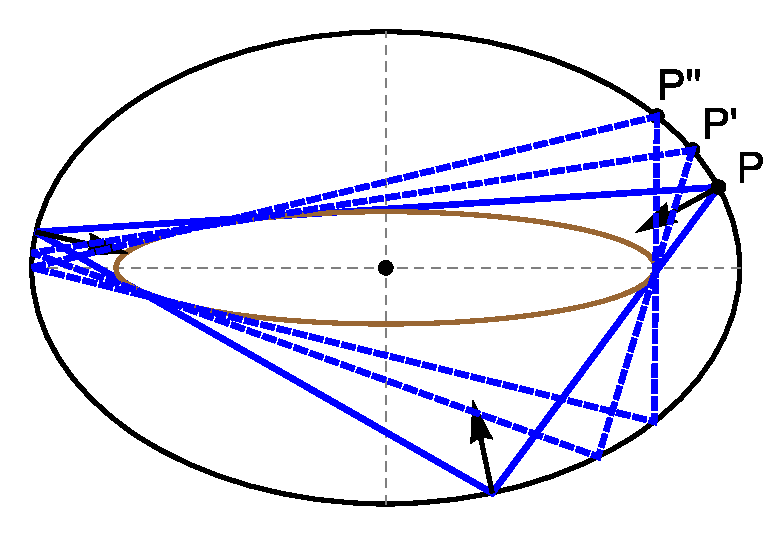
\includegraphics[width=.66\textwidth]{pics_eps_new/0090_three_orbits_proofs.eps}
    \caption{3-periodics (blue) in the Elliptic Billiard (EB, black): normals to the the boundary at vertices (black arrows) are bisectors. The family is constant-perimeter and envelopes a confocal Caustic (brown). This family conserves the ratio inradius-to-circumradius and has a stationary Mittenpunkt at the EB center. \textbf{Video}: \cite[PL\#01]{reznik2020-playlist-circum}.}
    \label{fig:three-orbits-proof}
\end{figure}

We have shown 3-periodics also conserve the Inradius-to-Circumradius\footnote{As does the Poristic Family \cite{gallatly1914-geometry}.} ratio which implies an invariant sum of cosines, and that their {\em Mittenpunkt}\footnote{Where lines drawn from each Excenter thru sides' midpoints meet.} is stationary at the EB center \cite{reznik2020-intelligencer}. Indeed many such invariants have been effectively generalized for $N>3$ \cite{akopyan2020-invariants,bialy2020-invariants}.

We have also studied the loci of 3-periodic Triangle Centers over the family: out of the first 100 listed in \cite{etc}, 29 sweep out ellipses (a remarkable fact on its own) with the remainder sweeping out higher-order curves \cite{garcia2020-ellipses}. Related is the study of  loci described by the Triangle Centers of the Poristic Triangle family \cite{odehnal2011-poristic}.

\textbf{Summary of the paper}: We first describe the {\em Circumbilliard}: the circumellipse associated with a generic triangle for which the latter is a 3-periodic. We then analyze the dynamic of geometry of Circumbilliards for triangles derived from the 3-periodic family such as the Excentral, Anticomplementary, Medial, and Orthic, as well as the loci swept by their centers. We then describe invariants detected for Circumconics and Inconics, namely:

\begin{itemize}
\item Proposition~\ref{prop:right-triangle} in Section~\ref{sec:cb_derived} describes regions of the EB which produce acute, right-triangle, and obtuse 3-periodics. 
\item Theorem~\ref{thm:poristic} in Section~\ref{sec:cb_derived}: The aspect ratio of Circumbilliards of the Poristic Triangle Family \cite{gallatly1914-geometry} is invariant. This is a family of triangle with fixed Incircle and Circumcircle.
    \item Theorem~\ref{thm:axis-ratio} in Section~\ref{sec:circumellipses}: The ratio of semi-axis of Circumellipses centered on the Incenter is invariant over the 3-periodic family. We conjecture this to be the case for a 1d-family of circumellipses.
    \item Theorem~\ref{thm:focal-ratio} in Section~\ref{sec:circumhyperbolae}: The focal lengths of two special circumhyperbola (Feuerbach and Excentral Jerabek) is constant over the 3-periodic family.
    \item Conjectures~\ref{conj:excIncX3} and \ref{conj:excIncX5} in Section~\ref{sec:inconic} claim the aspect ratios of two important Excentral Inconics are invariant. Candidate expressions are provided which match our experiments.
\end{itemize}

A reference table with all Triangle Centers, Lines, and Symbols appears in Appendix~\ref{app:symbols}. Videos of many of the experiments are assembled on Table~\ref{tab:playlist} in Section~\ref{sec:conclusion}.



